\documentclass[10pt,a4paper]{article}
\usepackage[margin=2.2cm]{geometry}
\usepackage{amsmath,amssymb,graphicx,booktabs,caption,float,xcolor,enumitem}
\usepackage[colorlinks=true,linkcolor=blue!50!black,citecolor=blue!50!black,urlcolor=blue!50!black]{hyperref}
\captionsetup{font=small,labelfont=bf}
\setlist{itemsep=1pt,topsep=3pt}
\graphicspath{{figures/}}
\newtheorem{hypothesis}{Hypothesis}

\title{\textbf{task003 and Object Placements side by side:}\\[2pt]
\textbf{the reading reversal and persistence in two tasks}}
\author{MA-CC project, LLM-free studies (Simulation 2)}
\date{23 October 2026}

\begin{document}
\maketitle

\begin{abstract}
\noindent
We compare the two phenomena of the LLM-free swarm simulator in two tasks: task003 (a team-allocation puzzle) and a
story from MuSR's Object Placements benchmark, each in a \emph{symmetric} setup (the agents can jointly prove the right
answer) and a \emph{no-proof} setup. The \textbf{reading reversal} appears in all four cases with the same qualitative
pattern. In Object Placements, however, the effects are about half as large, the symmetric crossover sits at lower memory,
and in the no-proof setup reading keeps amplifying the controller up to the largest reading depth.
\textbf{Persistence} differs. Without communication, after removal of the controller's facts, and with a frozen board,
both tasks behave alike. Under normal continuation, task003's effect stays flat for 100 time units while Object
Placements' fades by 30--60\%. Measurements on the stored runs show that the controller's facts keep circulating in Object
Placements but stop persuading. Each episode's board loses distinct controller facts by drift in both tasks, and only
Object Placements needs that variety, because its controller evidence is spread over many individually weak facts. We
state this and four further hypotheses, each with the measurement that supports it and the test that would decide it.
\end{abstract}

\section{What is compared}
A swarm of $N=24$ exact Bayesian agents shares a board. Each agent repeatedly reads $q$ of the 48 newest posts, forgets
each remembered fact at rate $\gamma=-\ln\rho$ (memory $\rho$ is the chance that a fact survives one time unit), votes
by sampling its exact posterior over three answers, and posts one fact that supports its vote. A false controller
posts true facts chosen to raise the probability of the wrong answer $A2$, until $t=30$. Every episode is run twice,
with the controller (\emph{false} arm) and without it (\emph{silent} arm), with shared random streams. The three
quantities are:
\begin{itemize}
\item the \textbf{controller effect} $G(\rho,q)$: the difference between the arms in the share of votes for $A2$
  (among agents who have voted), at $t=30$;
\item the \textbf{reading increment} $D(q_1\!\to\!q_2)=G(q_2)-G(q_1)$: positive when reading more helps the controller,
  negative when it protects the swarm;
\item the \textbf{effect after the controller stops}, $\delta(t)$ for $t>30$: the same difference over time, in four
  continuations: \emph{normal}; \emph{frozen board} (agents read only the board as it was at $t=30$, nobody posts);
  \emph{no communication} (no reading, no posting); and \emph{controller facts removed} (facts only the controller
  had are deleted from memories and board, then normal).
\end{itemize}
All simulation points use 1{,}000 paired episodes, with 95\% intervals. The runs are:
\begin{itemize}
\item task003 reversal: \texttt{2026-10-20\_sim2\_reading\_mechanism};
\item task003 persistence: \texttt{2026-10-20\_sim2\_persistence\_branches};
\item Object Placements reversal: \texttt{2026-10-22\_sim2\_op\_main};
\item Object Placements persistence: \texttt{2026-10-23\_sim2\_op\_post\_stop}.
\end{itemize}
The two tasks share every rule and parameter. Only the world and the setups differ.

\section{How the two tasks differ}
\label{sec:diff}
\begin{table}[h]
\centering\small
\resizebox{\linewidth}{!}{%
\begin{tabular}{@{}lll@{}}
\toprule
 & task003 & Object Placements \\
\midrule
what the puzzle is & who does which of 2 jobs, from 9 hidden skill numbers & where a person will look for an item, after 3 moves \\
possible states & 14{,}388, equally likely & 617{,}472 stories, weighted by the generator's probability \\
kind of fact & a skill level (``Alice's skill for the data pipeline is at least moderate'') & event or belief (``Casey did not see move 2'') \\
true facts in the story & 49 & 34 \\
answers & $A0$ (right), $A1$, $A2$ (controller's target) & $A0$ = Casey's belief (right), $A1$, $A2$ = where the keys are \\
agent facts: distinct / held twice & symmetric 18 / 6; no-proof 15 / 9 & same \\
symmetric: smallest proof of $A0$ from agent facts & \textbf{6 facts} (12 such proofs) & \textbf{3 facts} (2 such proofs) \\
single agent fact, median $P(A0\mid\{f\})$ & 0.36 (sym.), 0.35 (no-proof) & 0.33 = prior (both) \\
controller-only facts, median $P(A2\mid\{f\})$ & 0.42 (sym.), 0.35 (no-proof) & \textbf{0.33 = prior} (both) \\
controller-only facts neutral on their own & none & 30\% (sym.), 50\% (no-proof) \\
strongest controller-only fact / pair, $P(A2)$ & 0.59 / 0.73 & 0.49 / 0.55--0.57 \\
pair synergy among controller-only facts (mean) & $-0.007$, $-0.004$ & $-0.001$, $+0.002$ (none in either task) \\
symmetric: $A2$ pool alone, $P(A2)$ & 0.89 & 0.98 \\
no-proof: pool alone & (0.37, 0.26, 0.37) & (0.67, 0, 0.33): favours the truth \\
\bottomrule
\end{tabular}}
\caption{The two tasks. All quantities are computed from the worlds and setups alone, before any dynamics
(\texttt{task\_structure.py}). ``Controller-only'' facts are the controller's pool facts that no agent starts with. Pair
synergy is $P(A2\mid\{f,g\})-\tfrac13$ minus the sum of the two single-fact excesses over $\tfrac13$.}
\label{tab:diff}
\end{table}

\begin{figure}[h]
\centering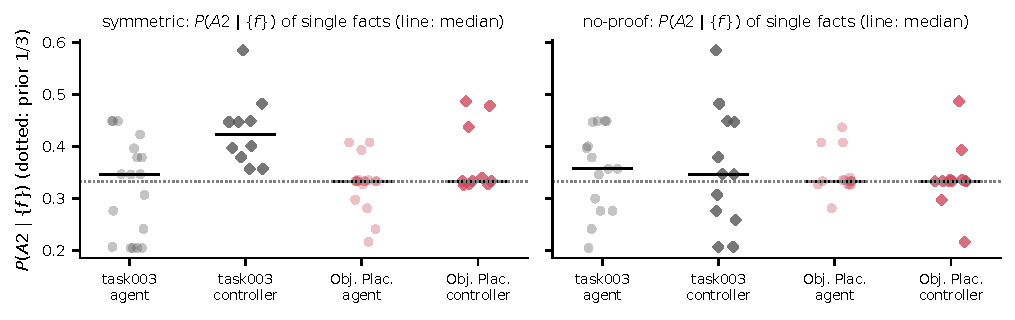
\includegraphics[width=\linewidth]{fig7_task_structure.pdf}
\caption{\textbf{How informative single facts are} (from the worlds alone). Each point is one fact: agent facts (circles)
and controller-only facts (diamonds). In task003, the controller's facts lean toward $A2$ on their own. In Object
Placements most facts of both kinds sit at the prior $1/3$: almost all evidence comes from combinations.}
\label{fig:structure}
\end{figure}

The difference that matters most below is \emph{where the evidence lives}. In task003 a single fact already carries
evidence: the controller's facts lean to $A2$ on their own (median 0.42 in the symmetric setup), and a proof of $A0$
needs 6 agent facts. In Object Placements a typical single fact says nothing (median exactly $1/3$). Evidence comes only
from combinations, a proof of $A0$ needs only 3 agent facts, and the controller's strongest single fact reaches 0.49.
Pairs add nothing beyond their single values on average in either task (Table~\ref{tab:diff}). So Object Placements'
controller evidence is \emph{diluted over many weak facts}, not concentrated in synergistic pairs.

% ======================================================================================================================
\section{Phenomenon I: the reading reversal}

\begin{figure}[h]
\centering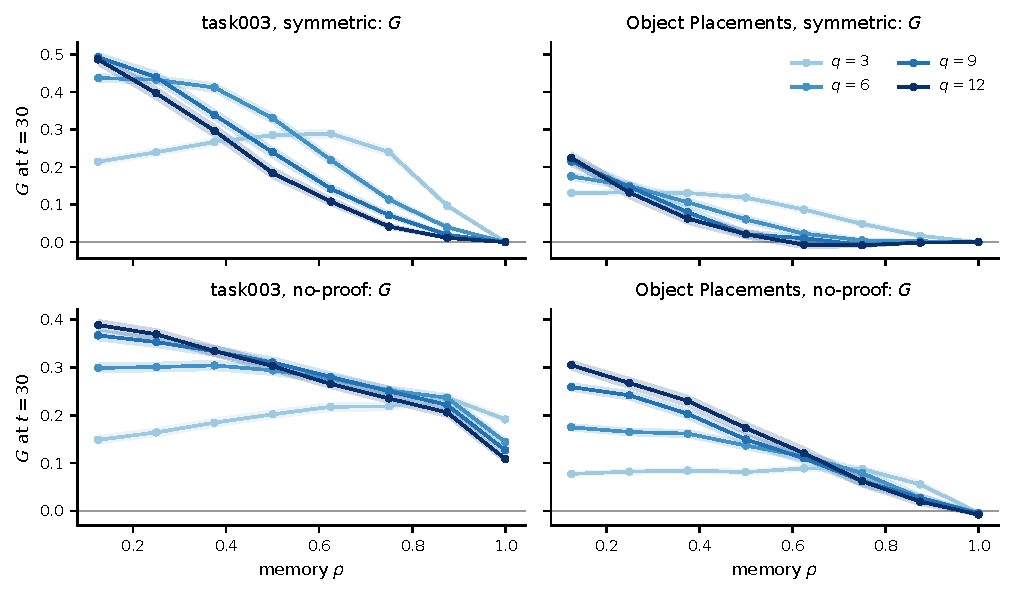
\includegraphics[width=\linewidth]{fig1_G_side_by_side.pdf}
\caption{\textbf{Controller effect $G$ at $t=30$} against memory $\rho$, for four reading depths $q$. Rows: setups.
Columns: tasks. Each row shares its vertical axis.}
\label{fig:G}
\end{figure}
\begin{figure}[h]
\centering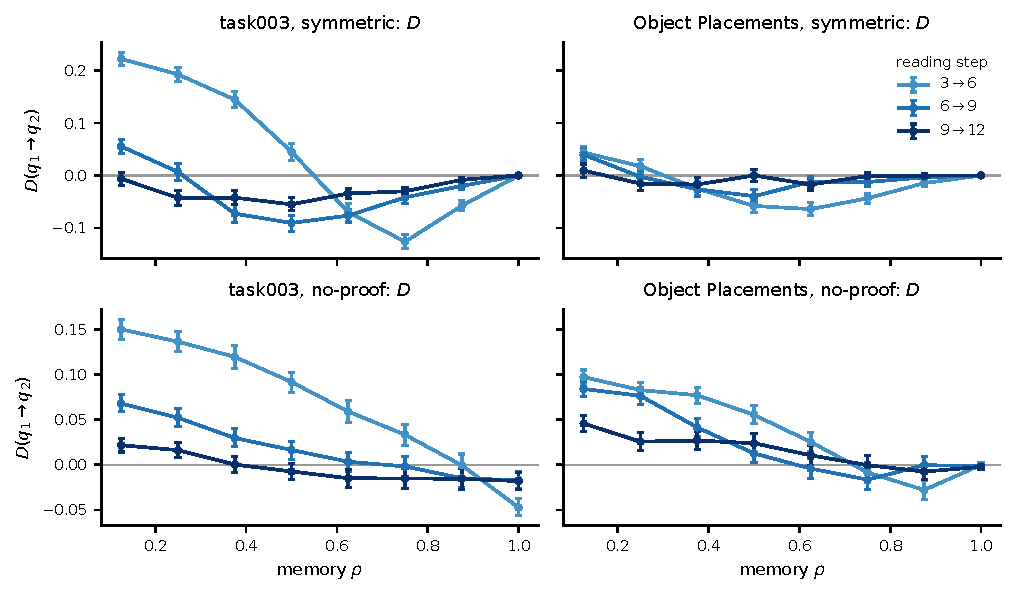
\includegraphics[width=\linewidth]{fig2_D_side_by_side.pdf}
\caption{\textbf{Reading increments $D$} (95\% intervals). Above zero, reading more helps the controller; below zero,
it protects the swarm.}
\label{fig:D}
\end{figure}
\begin{figure}[h]
\centering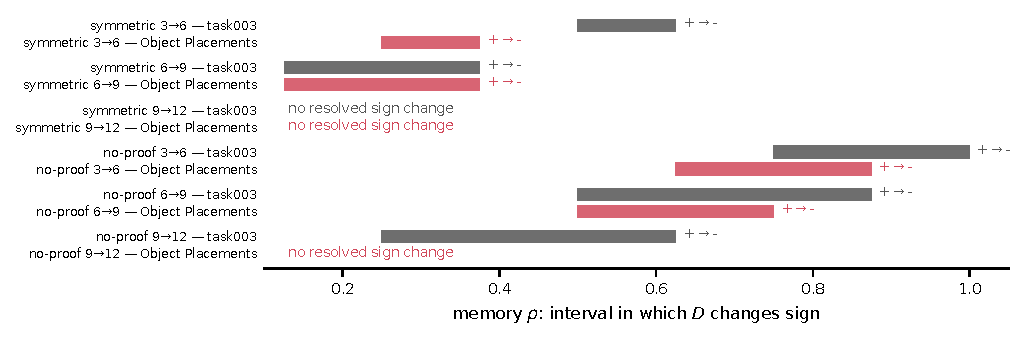
\includegraphics[width=\linewidth]{fig3_crossovers.pdf}
\caption{\textbf{Where the reversal happens:} the $\rho$ interval in which the resolved sign of $D$ changes, for each
setup and reading step (grey: task003; red: Object Placements).}
\label{fig:cross}
\end{figure}

\paragraph{What is the same.} The reversal exists in both setups of both tasks (Figs.~\ref{fig:G}--\ref{fig:cross}). At
low memory reading more helps the controller; at high memory it protects the swarm. In both tasks the no-proof setup
reverses at higher memory than the symmetric one, and in the no-proof setup the crossover falls as $q$ grows ($3\to6$
before $6\to9$). At $\rho=1$ the symmetric swarm proves the right answer in both tasks and $G=0$.

\paragraph{What is different.}
\begin{enumerate}
\item \textbf{Size.} Object Placements' effects are about half of task003's. At $\rho=0.125$, $q=6$, $G$ is 0.18 against
  0.44 (symmetric) and 0.17 against 0.37 (no-proof).
\item \textbf{Symmetric crossover.} $D(3\to6)$ changes sign between $\rho=0.25$ and $0.375$ in Object Placements,
  against $0.5$--$0.625$ in task003. The $6\to9$ crossover is the same in both tasks ($0.125$--$0.375$).
\item \textbf{No-proof, deep reading.} In task003 the increments shrink quickly with $q$, and $9\to12$ is resolved negative
  from $\rho=0.625$. In Object Placements $6\to9$ is about as large as $3\to6$ at low memory, and $9\to12$ is never
  resolved negative: reading more keeps helping the controller.
\end{enumerate}

\paragraph{Hypotheses.}
\begin{hypothesis}[size]
The effect is smaller in Object Placements because the controller has no individually strong facts. Its best single fact
reaches $P(A2)=0.49$, against 0.59 in task003, and most of its facts are neutral alone (Table~\ref{tab:diff}). An agent
that reads a few controller facts is moved less.
\end{hypothesis}
\begin{hypothesis}[symmetric crossover]
Reading protects the symmetric swarm by letting agents assemble a proof of $A0$. In Object Placements a proof needs only 3
agent facts, against 6 in task003. A 3-fact proof is assembled, and survives forgetting, at shorter memory: a proof of $k$
facts survives a time $t$ without rereading with probability $e^{-k\gamma t}$. Reading therefore becomes protective at
lower $\rho$. \emph{Test:} the share of agents holding a complete proof at $t=30$, against $\rho$ and $q$, in both tasks
(planned analysis A2--A3).
\end{hypothesis}
\begin{hypothesis}[no-proof, deep reading]
With weak, diluted controller evidence, an agent needs several \emph{distinct} controller facts in one memory to be moved.
More reading gathers more of them, so amplification keeps growing with $q$. In task003 one strong controller fact
already gives most of the push, so the gain from reading saturates early. \emph{Test:} the push of a read, $P(A2\mid
\text{read})$, against the number of distinct controller facts it contains, in both tasks.
\end{hypothesis}

% ======================================================================================================================
\section{Phenomenon II: persistence}

\begin{figure}[h]
\centering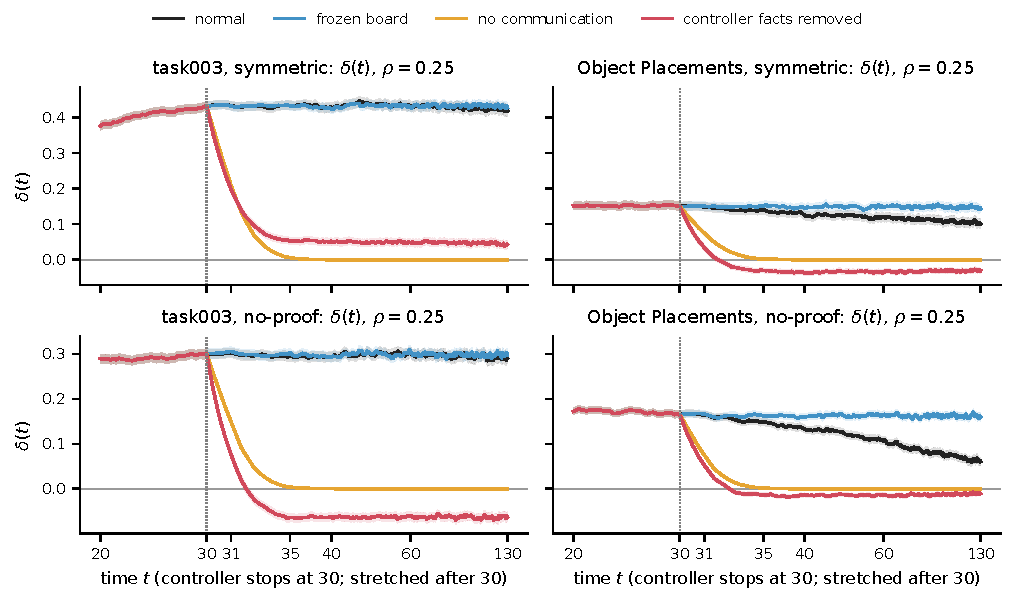
\includegraphics[width=\linewidth]{fig4_persistence_rho025.pdf}
\caption{\textbf{After the controller stops, $\rho=0.25$} ($q=6$; 95\% bands). Rows: setups. Columns: tasks. The time
axis is stretched after $t=30$.}
\label{fig:p025}
\end{figure}
\begin{figure}[h]
\centering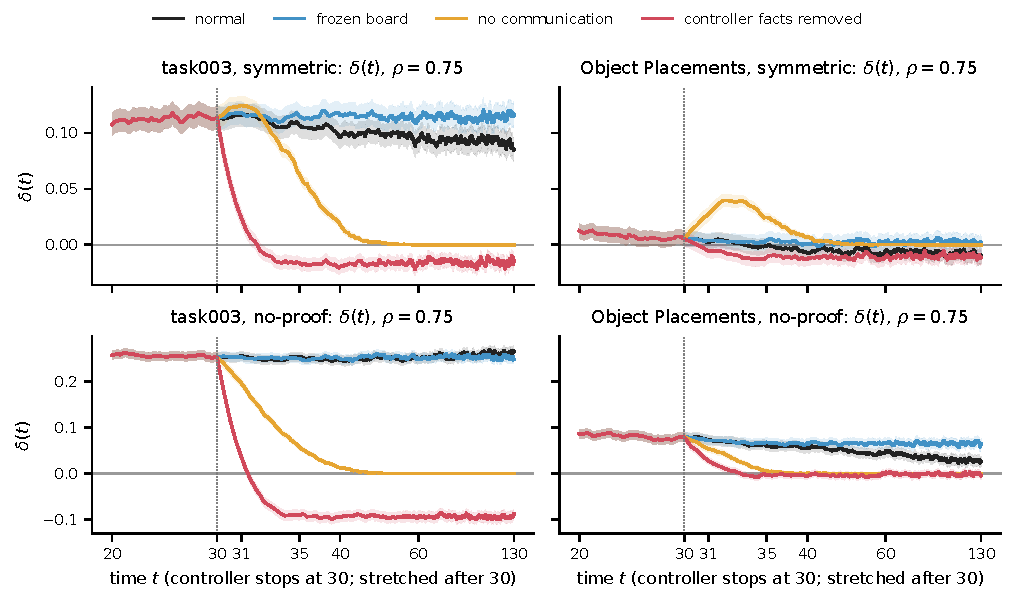
\includegraphics[width=\linewidth]{fig5_persistence_rho075.pdf}
\caption{\textbf{After the controller stops, $\rho=0.75$.} In Object Placements' symmetric setup there is almost no effect to
persist ($G\approx0$ at this memory).}
\label{fig:p075}
\end{figure}

\paragraph{What is the same} (Figs.~\ref{fig:p025}--\ref{fig:p075}).
\begin{itemize}
\item \textbf{No communication:} the effect vanishes on the memory time scale. The half-time is 1.0 time unit at
  $\rho=0.25$ in all four cases; at no-proof $\rho=0.75$ it is 2.5 in task003 and 2.0 in Object Placements.
\item \textbf{Controller facts removed:} the effect collapses within about 1 time unit to a small residual.
\item \textbf{Frozen board:} the effect stays flat to $t=130$ in every case.
\end{itemize}

\paragraph{What is different.}
\begin{enumerate}
\item \textbf{Normal continuation fades in Object Placements} (from $t=30$ to $130$):
  \begin{itemize}
  \item no-proof $\rho=0.25$: $0.165\to0.061$;
  \item no-proof $\rho=0.75$: $0.079\to0.026$;
  \item symmetric $\rho=0.25$: $0.150\to0.100$.
  \end{itemize}
  In task003 the same cells stay flat: $0.30\to0.29$, $0.25\to0.26$ and $0.43\to0.42$. M4 predicted this difference
  before the Object Placements data existed (pre-registration commit \texttt{09208a7}).
\item \textbf{Sign of the residual after removal, symmetric $\rho=0.25$:} $+0.04$ in task003 (lasting damage), $-0.03$
  in Object Placements.
\item \textbf{A transient rise without communication} in the symmetric setups at $\rho=0.75$. When reading stops, $\delta$
  first rises before decaying: by about 0.04 in Object Placements, from a near-zero start, and from 0.11 to 0.125 in
  task003.
\end{enumerate}

\begin{figure}[h]
\centering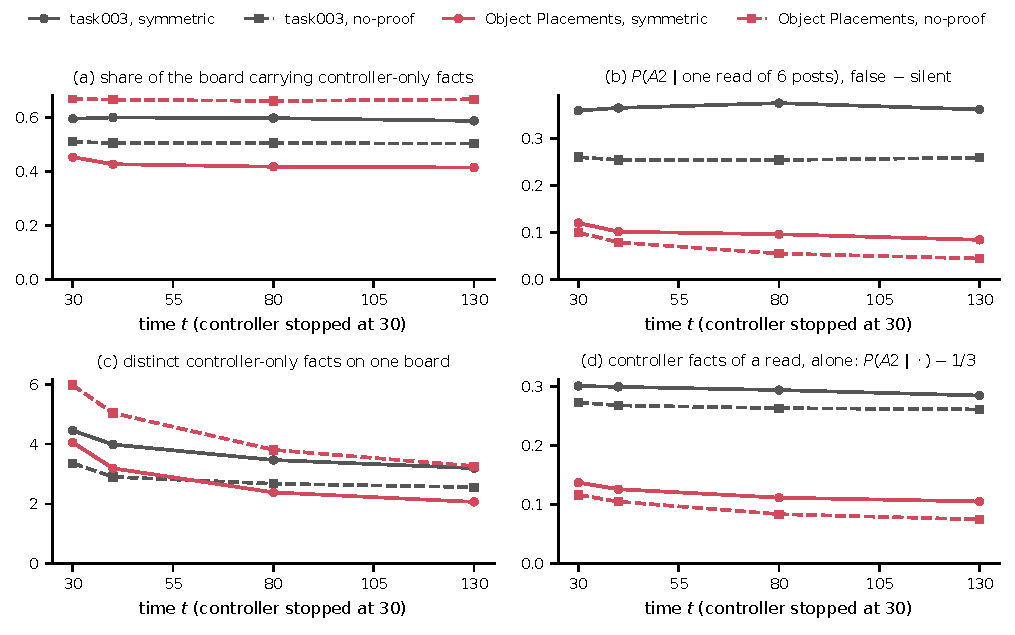
\includegraphics[width=\linewidth]{fig6_mechanism_after_stop.pdf}
\caption{\textbf{Why the effect fades in Object Placements} (false arm, normal continuation, $\rho=0.25$; averages over
episodes from the stored posts and memories). (a) The controller's facts keep circulating at a constant share of the board
in both tasks. (b) But the push of a typical read toward $A2$ (false minus silent arm) stays constant in task003 and falls
in Object Placements. (c) Within each episode, the number of distinct controller facts on the board falls in both tasks:
drift. (d) The push of the controller facts in a read, taken alone, falls only in Object Placements.}
\label{fig:mech}
\end{figure}

\paragraph{Explanation of the fading (supported by measurements).} Two candidate causes were tested on the stored runs
(Fig.~\ref{fig:mech}). \emph{Circulation} would mean the controller's facts die out. \emph{Persuasion} would mean they
still circulate but push less.
\begin{itemize}
\item Circulation does not change: controller-only facts occupy a constant share of the board (no-proof $\rho=0.25$:
  0.67 at $t=30$ and at $t=130$), and their number per agent memory falls only moderately in both tasks.
\item Persuasion changes. The extra push of a read in the false arm falls from 0.10 to 0.045 in Object Placements and
  stays at 0.26 in task003 (no-proof $\rho=0.25$).
\item The \emph{mix} of controller facts, judged one fact at a time, does not change (share-weighted single-fact
  $P(A2)$: 0.36 at both times in Object Placements). What changes is their \emph{variety within an episode}: from 6.0 to
  3.3 distinct controller facts per board in Object Placements, and from 3.4 to 2.6 in task003.
\end{itemize}

\begin{hypothesis}[persistence needs concentrated evidence]
After the controller stops, its facts are reposted by agents and drift like neutral alleles. Within each episode drift
removes variety: a few controller facts take over the board while their partners disappear. Averaged over episodes the
shares stay constant. In task003 this does not matter, because each controller fact pushes on its own, so the imprint
persists. In Object Placements the push needs several distinct weak facts in the same read, so losing variety weakens it,
and the effect fades on the time scale of drift.
\end{hypothesis}
Three checks agree with this hypothesis.
\begin{itemize}
\item \textbf{Frozen board.} The frozen board stays flat in Object Placements too. With no posting there is no drift,
  and the variety present at $t=30$ is kept.
\item \textbf{M4.} M4 reproduces the fading. It contains drift of integer fact counts and the exact evidence rule, and
  nothing task-specific.
\item \textbf{Fading by cell.} The fading is strongest where the controller started with most variety: no-proof, 6
  distinct facts per board.
\end{itemize}
One quantitative failure is open: M4 relaxes too slowly at no-proof $\rho=0.75$ (half-time 75 against 27).
\emph{Decisive test:} recompute panel (b) after shuffling posts between episodes while keeping each fact's overall share.
This restores variety without changing the shares, so the fading should disappear in Object Placements and nothing
should change in task003.

\begin{hypothesis}[residual after removal]
A positive residual means that the controller's earlier activity damaged the swarm's own evidence for good. In task003's
symmetric setup, the false arm ends up with about 2.4 fewer distinct agent facts in circulation than the silent arm. In
Object Placements the gap is about 0.8. So removing the controller's facts leaves lasting damage in task003 ($+0.04$) but
not in Object Placements ($-0.03$).
\end{hypothesis}

\begin{hypothesis}[transient rise without communication]
When reading stops, memories decay fact by fact. A proof of $A0$ breaks as soon as any one of its $k$ facts is forgotten
(rate $k\gamma$). A single controller fact is lost at rate $\gamma$. In the symmetric setups at $\rho=0.75$, both arms
start with many proofs. In the false arm, proofs break faster than controller facts disappear, so for a few time units
more agents are left with controller facts and no proof, and $\delta$ rises. It then decays as everything is forgotten.
\emph{Test:} the share of agents with a complete proof and the share with a controller fact, over time in the
no-communication branch.
\end{hypothesis}

% ======================================================================================================================
\section{Summary}
\begin{table}[h]
\centering\small
\resizebox{\linewidth}{!}{%
\begin{tabular}{@{}llll@{}}
\toprule
observation & task003 & Object Placements & explanation (status) \\
\midrule
reversal in both setups & yes & yes & finite-swarm fact dynamics (M4; tested, pre-registered on Obj.\ Plac.) \\
effect size ($G$, $q=6$, $\rho=0.125$) & 0.44 / 0.37 & 0.18 / 0.17 & weak controller facts (Hyp.~1; consistent, untested) \\
symmetric $3\to6$ crossover & 0.5--0.625 & 0.25--0.375 & 3-fact against 6-fact proofs (Hyp.~2; to test) \\
no-proof: reading keeps amplifying & no & yes & diluted controller evidence (Hyp.~3; to test) \\
persists, normal continuation & flat & fades 30--60\% & drift removes variety (Hyp.~4; supported, shuffle test pending) \\
frozen board / no comm. / removal & flat / $\to0$ / residual & same & frozen: no drift; no comm.: forgetting \\
residual sign after removal (sym.\ 0.25) & $+0.04$ & $-0.03$ & lasting extinction damage (Hyp.~5; consistent) \\
transient rise without communication & small & 0.04 & proofs break faster than single facts (Hyp.~6; to test) \\
\bottomrule
\end{tabular}}
\caption{Same and different, with the proposed explanation and its status.}
\label{tab:summary}
\end{table}

The general lesson is that the same collective dynamics (copying, forgetting, drift and extinction of facts) produce
different outcomes depending on \emph{how evidence is distributed over facts}. Concentrated evidence persists; diluted
evidence fades under drift. Small proofs make reading protective at shorter memory. This is the evidence layer that the
planned theory (analyses A1--A4) must make explicit.

\paragraph{Reproducibility.} Scripts in \nolinkurl{analysis/theory/reports/2026-10-23_task_comparison/}:
\begin{itemize}
\item \nolinkurl{task_structure.py}: Table~\ref{tab:diff} and Fig.~\ref{fig:structure};
\item \nolinkurl{carrier_after_stop.py}, \nolinkurl{board_persuasion.py}, \nolinkurl{context_value.py} and
  \nolinkurl{ctrl_diversity.py}: Fig.~\ref{fig:mech};
\item \nolinkurl{make_figures.py}: all figures.
\end{itemize}
Simulation data sources are listed in Section~1.


\section*{Addendum, 24 October 2026}
Added after Phase C of the theory work (\nolinkurl{analysis/theory/phaseC/phaseC_results.md}). Nothing above was
rewritten.
\begin{enumerate}
\item \textbf{Hypothesis 4 is rejected.} Each episode was continued from its stored state at $t=30$ under three posting
  rules:
  \begin{itemize}
  \item new posts copy a random board post (neutral);
  \item new posts are a random fact of the poster's memory (neutral, two reservoirs);
  \item the simulator's own rule: post a fact that supports one's vote in context.
  \end{itemize}
  Only the real rule reproduces both task003's persistence and Object Placements' fading. It passes the pre-registered
  checks in 7 of 7 cells; the two neutral rules pass 0/7 and 2/7. Neutral posting from memories keeps the effect
  \emph{from} fading in Object Placements (retained 0.73 against 0.37 at no-proof $\rho=0.25$). So the fading is caused
  by the \emph{selection} of the posting rule, not by drift. The loss of variety in Fig.~\ref{fig:mech}(c) is a
  consequence of that selection.
\item \textbf{Revised explanation.} A held controller fact is reposted only if it supports its holder's current vote in
  context. That happens 0.78--0.82 of the time in task003 and 0.53--0.56 in Object Placements ($\rho=0.25$). In Object
  Placements single facts support a vote only in particular combinations, so the controller's facts drain once nothing
  replenishes them. The task-structure contrast of Section~\ref{sec:diff} is the right variable; the mechanism is
  selection.
\end{enumerate}

\end{document}
